\section{Solar Coordinates}
\label{sec:coords}

The \package{sunpy.coordinates} subpackage provides support for representing and transforming solar-centric coordinates. 
These coordinates may represent events (e.g. flares), feature on or above the Sun (e.g. magnetic loops), or  the position of structures traveling throughout the heliosphere such as coronal mass ejections.
The package currently supports many of the most widely used Sun-centered coordinate frames including Helioprojective Cartesian (HPC), Heliographic Carrington (HGC), Heliographic Stonyhurst (HGS),  as well as Heliocentric Aries Ecliptic (HAE), Heliocentric Cartesian (HCC) and Heliocentric Earth Equatorial (HEEQ). 
For more information about these coordinates frames \citep[see][]{2006A&A...449..791T}.
The functionality provided in this package is built on top of and integrates with the \package{astropy.coordinates} framework \citep[see Section 3.3 of][]{astropy2018}.

An important feature of some of these solar coordinate frames is that they are observer-dependent, meaning that they are not fully defined without also specifying the location of the observer.
The HPC frame, in particular, which is the most widely used coordinate frame for images of the Sun, places the origin of the frame at the observed center of the solar disk.
This means that these observer-dependent frames have axes that change orientation depending on the location of the observer, and thus the observer location is necessary to fully define the frame.
In order to accommodate this, all observer-dependent solar coordinates add an observer attribute with the observer coordinate.
Since many observations of the Sun take place from or near the Earth, it is frequently an adequate approximation to use the Earth's location as the observer.

The observer-independent coordinate frames (HAE, HEEQ, HGC, and HGS) are useful for specifying the locations of features on the Sun or objects (e.g., spacecraft) in interplanetary space.
The commonly-used HGS frame is of particular note because it transforms in a straightforward manner to and from the Heliocentric Celestial Reference System (HCRS).
This transformation consists of the combination of two rotation angles: the time-independent angle between the Sun's rotation axis and the HCRS celestial pole \citep[see][]{2007CeMDA..98..155S} and the time-dependent angle of the central meridian (as seen from Earth) relative to the vernal equinox.
This transformation provides the link from the frames defined in \package{sunpy.coordinates} with those defined in \package{astropy.coordinates}, allowing any solar frame to be transformed to and from celestial coordinate frames (\autoref{fig:transform_graph}).
%In fact, HAE is actually implemented in \package{astropy.coordinates}, but the shared framework means that it can be used seamlessly in \sunpypkg.
The functionality provided by  \package{sunpy.coordinates} subpackage has been extensively tested and agrees with published values in the \textit{Astronomical Almanac} to a precision of hundredth of an arcsecond for apparent right ascension.

\begin{figure}
    \centering
    \includegraphics[width=0.75\textwidth]{figures/sunpy_frames.pdf}
    \caption{Graph of the coordinate frames accessible through \package{sunpy.coordinates}, and how they transform between each other.
    The frames within the blue box are implemented in \package{astropy.coordinates}, but in the shared framework, any frame can be transformed to any other frame in this graph.}
    \label{fig:transform_graph}
\end{figure}

A few example applications of the functionality provided by \package{sunpy.coordinates} are shown in \autoref{fig:coordinates_examples}. 
The first panel shows magnetic field line extrapolations projected onto an SDO/AIA 171\AA{} image of an active region.
The center and rightmost panels of \autoref{fig:coordinates_examples} make use of functions in \package{sunpy.coordinates} to obtain the apparent (light-travel time-corrected) location of solar-system bodies and overlay them on images of the Sun in solar coordinate frames.
Support is  provided for querying ephemeris information from a few different sources including the active ephemeris in \package{astropy.coordinates}, JPL ephemeris, and JPL HORIZONS\footnote{\url{https://ssd.jpl.nasa.gov/?horizon}} which also provides ephemeris information of spacecraft such as SDO, SOHO, and the two STEREO spacecraft.

\begin{figure}
    \gridline{\fig{figures/fig_fieldlines_aia.pdf}{0.3\textwidth}{(a)}
              \fig{figures/fig_venus_transit.pdf}{0.3\textwidth}{(b)}
              \fig{figures/fig_coronagraph_starfield.pdf}{0.3\textwidth}{(c)}
              }
    \caption{Several example use cases of the coordinate machinery provided by the \package{sunpy.coordinates} subpackage.
    (a) Magnetic field lines traced from a potential field extrapolation overlaid on an SDO/AIA 171 \AA{} AIA observation of an active region from 2019 March 10 00:00:09 UTC.
    The field extrapolation was computed with \package{pfsspy} \citep{david_stansby_2019_3237053}.
    (b) The Venus transit as viewed by SDO/AIA in 1600 \AA. The predicted position of Venus is overplotted in the helioprojective coordinate frame of the AIA image.
    (c) A coronagraph image of the solar corona as observed by STEREO-A COR-2. The predicted positions of stars from the Gaia DR2 catalog (shown as circles) as well as Mars (shown as a box) are overplotted in the helioprojective coordinate frame of the image.}
    \label{fig:coordinates_examples}
\end{figure}

\subsection{Differential Rotation}
\label{sec:differential_rotation}

%1-2 sentences intro; 1-2 sentences describing what is new; 1 sentence that acknowledges the figure.
% Can delete the first two sentences if the background info feels unnecessary

When analyzing the dynamics of features on the solar disk, it is important to account for variations due to the apparent rotation of the Sun.
There are two important effects, the apparent rotation of the Sun as seen from platforms that are orbiting around the Sun such as the Earth and solar differential rotation or the latitudinally-varying rotation rate due to the non-rigidity of the solar interior \citep[see][]{Beck2000}.
The \package{sunpy.physics.differential\_rotation} subpackage provides tools for correctly accounting for both of these effects on solar coordinates. 
\autoref{fig:diff_rot} shows an example of this functionality applied to a SDO/AIA 1600 \AA{} image which features two prominent active regions. The bottom panel shows the predicted image including differential rotation and the apparent solar rotation due to the observers orbit. This predicted image can be compared to an actual later image by SDO/AIA 1600 \AA{}.

\begin{figure}
    \center
    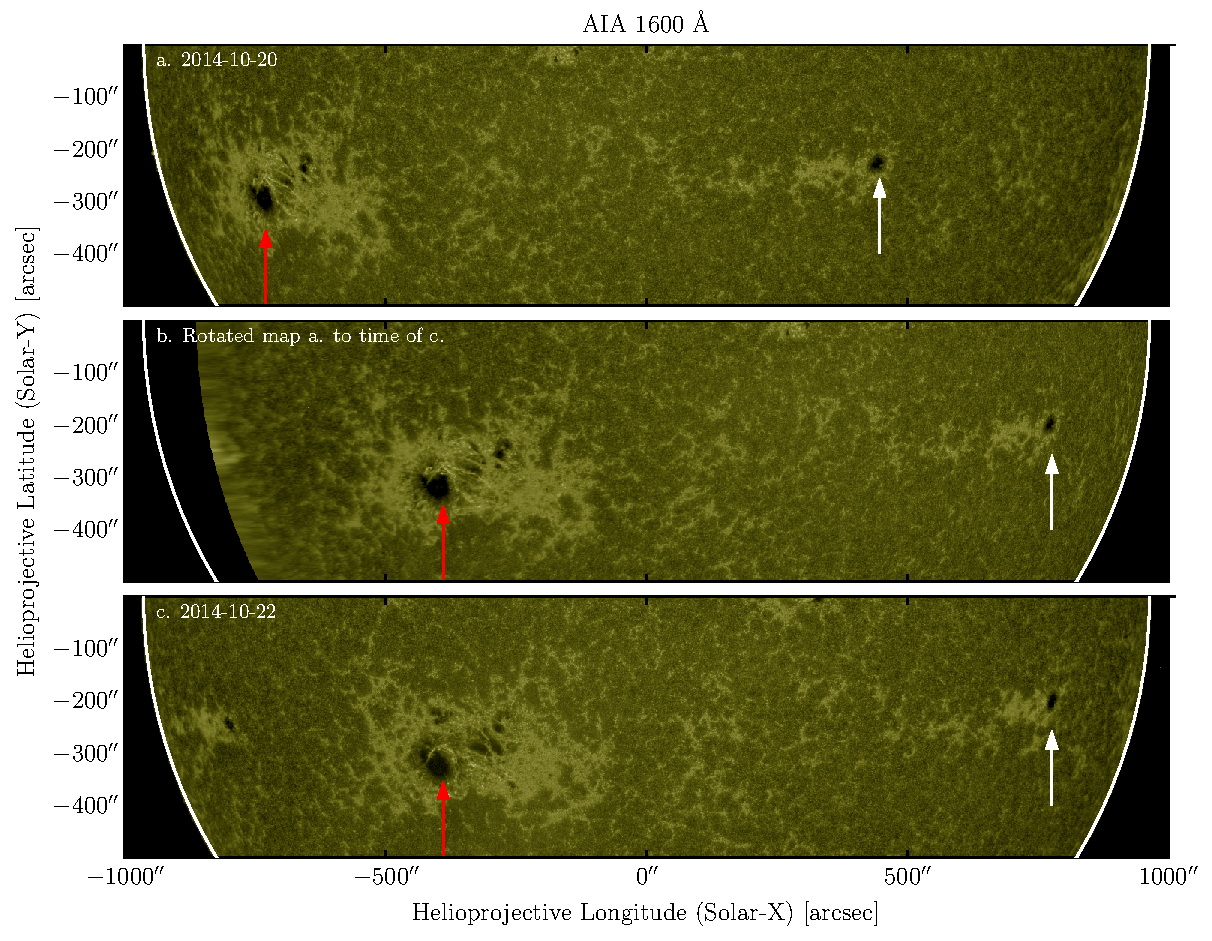
\includegraphics[width = 0.8\textwidth]{figures/fig_diff_rot_1600.pdf}
    \caption{The effects of differential rotation.
    Panels (a) show the Sun as observed by SDO/AIA in 1600~\AA\.
    A large and small sunspot group is highlighted by a red and white arrow respectively. 
    Panel (b) shows the predicted image after having been rotated two days into the future.
    Panel (c) shows the actual observation on the day of panel (b) which compares well to the predicted image neglecting the magnetic evolution of the sunspot groups.}
    \label{fig:diff_rot}
\end{figure}
